% !TeX program = pdflatex
% Prefer the repository's template files whether compilation starts from the
% repository root or from this directory.
\makeatletter
\def\input@path{{paper/}}
\makeatother
\IfFileExists{paper/jmlr.cls}
{\documentclass[mlabstract]{paper/jmlr}}
{\documentclass[mlabstract]{jmlr}}

% Watermark for review. Remove these four commands for the camera-ready version.
\usepackage[hpos=300px,vpos=70px]{draftwatermark}
\SetWatermarkText{\test}
\SetWatermarkScale{1}
\SetWatermarkAngle{0}

% The jmlr class automatically loads amsmath, amssymb, natbib, graphicx,
% url, and algorithm2e, as required by the submission instructions.
\graphicspath{{generated/figures/}{paper/generated/figures/}}

% Do not change the proceedings metadata below.
\jmlrvolume{}
\firstpageno{1}
\editors{List of editors' names}
\jmlryear{2026}
\jmlrworkshop{Symmetry and Geometry in Neural Representations}

\title[Weight-space gradient descent induces activity descent]
{Weight-space gradient descent induces approximate activity descent,
making learning rules testable}
% \title[Activity descent in neural networks]{Activity descent in neural networks: a testable prediction for biological learning rules}

\newcommand{\vW}{\mathbf{W}}
\newcommand{\vA}{\mathbf{A}}
\newcommand{\vy}{\mathbf{y}}
\newcommand{\vh}{\mathbf{h}}
\newcommand{\vs}{\mathbf{s}}
\newcommand{\vu}{\mathbf{u}}
\newcommand{\vv}{\mathbf{v}}
\newcommand{\grad}{\nabla_{\!\vW_{\leq\ell}}}
\newcommand{\loss}{\mathcal{L}}

\begin{document}

\maketitle

\begin{abstract}
  A central question in neuroscience is whether biological neural networks optimise a loss function by adjusting synaptic weights -- and if so, by what rule.
  Candidate rules are difficult to test because synaptic weights cannot be measured at scale in behaving animals, whereas neural \emph{activities} can be recorded across learning.
  This raises the question: if a network performs gradient descent on its weights, what should we see in its activities?
  Here we show that weight-space gradient descent induces kernel-filtered activity descent; when the kernel is approximately diagonal, each neuron follows its own loss gradient.
  We validate this prediction in ANNs of moderate width and depth, showing that indeed changes in neural activities are correlated with their loss gradients.
  The same relationship can and should be tested in biological neural networks with existing experimental techniques.
\end{abstract}

\begin{keywords}
  neural activity, activations, gradient descent, learning rules, neuroscience
\end{keywords}

\paragraph{Weight-space descent and observable activity.}
Neuroscience has long sought to understand learning rules in biological neural networks, and the success of ANNs trained by gradient descent has renewed interest in finding commensurate rules in the brain \citep{richardsDeepLearningFramework2019}.
A key challenge, however, is that synaptic weights are not directly observable in vivo; modern neuroscience experiments measure neural activity instead.
\cite{richardsStudyPlasticityHas2023} proposed validating gradient-based learning rules by observing how neural activity changes during learning, but implicitly assumed a link between gradient descent on synaptic weights and the resulting activity changes.
We formalize that link here, showing that weight-space gradient descent induces kernel-filtered descent in neural activations.

\vspace{-0.5em}
\paragraph{Setup and derivation.}
Consider a feedforward network with layers $\ell=1,\ldots,L$, weights $\vW$, and neural activities $A_i^{(\ell)}(\vW)$, trained to minimise a loss $\loss$.
Let $\mathcal N_\ell:=\{1,\ldots,n_\ell\}$ index the neurons in layer~$\ell$, let $\mathcal P_r$ index the scalar weights in layer~$r$, and define the upstream parameter-index set $\mathcal P_{\leq\ell}:=\bigcup_{r=1}^{\ell}\mathcal P_r$.  Thus $i,j,k\in\mathcal N_\ell$ index neurons in a fixed layer, whereas $\alpha\in\mathcal P_{\leq\ell}$ indexes a scalar upstream weight $W_\alpha$.
We write $\vW_{\leq\ell}:=(W_\alpha)_{\alpha\in\mathcal P_{\leq\ell}}$ for the corresponding block of weights.

In gradient descent, every weight is updated simultaneously:
%
\begin{equation}
  \Delta W_\alpha = -\eta\,\frac{\partial \loss}{\partial W_\alpha}\,,
  \qquad \forall\;\alpha\in\mathcal P_{\leq L}.
\end{equation}
%
What is the induced change in the activity of neuron $i$ in layer~$\ell$?  Because $A_i^{(\ell)}$ depends only on $\vW_{\leq\ell}$, if the activity map is twice differentiable with bounded second derivatives along the update segment, Taylor expansion around the pre-update weights $\vW_t$ gives
\[
  \Delta A_i^{(\ell)}
  \;:=\; A_i^{(\ell)}(\vW_t + \Delta\vW) - A_i^{(\ell)}(\vW_t)
  \;=\; \nabla_{\!\vW_{\leq\ell}} A_i^{(\ell)}(\vW_t)^{\!\top}\,\Delta\vW_{\leq\ell}
  + O\!\left(\lVert\Delta\vW_{\leq\ell}\rVert^2\right).
\]
Since $\Delta\vW=O(\eta)$, substituting $\Delta W_\alpha = -\eta\,\partial\loss/\partial W_\alpha$ gives
%
\begin{equation}\label{eq:approx}
  \Delta A_i^{(\ell)}
  \;\approx\; -\eta \sum_{\alpha\in\mathcal P_{\leq\ell}} \frac{\partial A_i^{(\ell)}}{\partial W_\alpha}\,\frac{\partial \loss}{\partial W_\alpha}\,,
\end{equation}
%
where all derivatives are evaluated at $\vW_t$ and the omitted remainder is $O(\eta^2)$.
For piecewise-linear activations such as ReLU, this statement applies when the step is small enough that no unit changes activation status, so the network remains within a single smooth piecewise-polynomial region of weight space.
% Higher-order cross-layer terms generally remain when weights in multiple layers are updated simultaneously (e.g.\ contributions of the form $\Delta\vW^{(2)}\Delta\vW^{(1)}\vA^{(0)}$); these terms are $O(\eta^2)$.
%
In a sequential feedforward network (one without skip or residual connections), the effect of any weight indexed by $\mathcal P_{\leq\ell}$ on the loss passes entirely through the activities of layer~$\ell$.
This allows us to use the chain rule to write the effect on the loss, $\partial \loss/\partial W_\alpha$, in terms of the activities at layer~$\ell$:
\begin{equation}\label{eq:chain}
  \Delta A_i^{(\ell)}
  \;\approx\; -\eta \sum_{\alpha\in\mathcal P_{\leq\ell}} \frac{\partial A_i^{(\ell)}}{\partial W_\alpha}\,\left[ \sum_{k\in\mathcal N_\ell} (\partial \loss/\partial A_k^{(\ell)})\,(\partial A_k^{(\ell)}/\partial W_\alpha)\right],
\end{equation}
Exchanging the sums yields
%
\begin{equation}\label{eq:main}
  \boxed{\;\Delta A_i^{(\ell)} \;\approx\; -\eta \sum_{k\in\mathcal N_\ell} \Phi^{(\ell)}_{ik}\;\frac{\partial \loss}{\partial A_k^{(\ell)}}\;,}
\end{equation}
%
where
%
\begin{equation}\label{eq:kernel}
  \Phi^{(\ell)}_{ik}
  \;:=\; \sum_{\alpha\in\mathcal P_{\leq\ell}} \frac{\partial A_i^{(\ell)}}{\partial W_\alpha}\,\frac{\partial A_k^{(\ell)}}{\partial W_\alpha}
  \;=\; \grad A_i^{(\ell)} \cdot \grad A_k^{(\ell)}
\end{equation}
%
is a Gram matrix defined on the activities within each layer, and $\partial \loss/\partial A_k^{(\ell)}$ is the full backpropagated loss gradient -- a sufficient statistic that compresses everything downstream layers contribute to the weight updates affecting layer~$\ell$.
In vector form, $\Delta\vA^{(\ell)} \approx -\eta\,\Phi^{(\ell)}\,\nabla_{\!\vA^{(\ell)}}\loss$: gradient descent in weight space induces \emph{kernel descent} within each layer of activity space.
It holds for any differentiable sequential feedforward network;
Architectures with skip connections require additional treatment, as weights can influence the loss through paths that bypass intermediate layers.

\vspace{-0.5em}
\paragraph{Relation to the neural tangent kernel.}
The first-order approximation we study should be familiar to those acquainted with the neural tangent kernel (NTK) \citep{jacotNeuralTangentKernel2018}.
The kernel $\Phi^{(\ell)}$ is a layer-wise analogue of the empirical neural tangent kernel (NTK) for finite-width networks \citep{leeWideNeuralNetworks2020}.

\vspace{-0.5em}
\paragraph{Self-terms drive each neuron toward its loss gradient; cross-terms interfere.}
The diagonal element \smash{$\Phi^{(\ell)}_{ii}=\lVert\grad A_i^{(\ell)}\rVert^2$} collects contributions from \emph{all} weights that influence neuron $i$.
Because $\Phi^{(\ell)}_{ii}\ge 0$, the self-term update is aligned with $-\partial \loss/\partial A_i^{(\ell)}$: each such neuron's activity moves down its own loss gradient, with an effective learning rate $\eta\,\Phi^{(\ell)}_{ii}$ that grows with the depth and width of its input pathways.

The off-diagonal elements $\Phi^{(\ell)}_{ik}=\grad A_i^{(\ell)}\cdot\grad A_k^{(\ell)}$ for $k\neq i$ couple neurons \emph{within the same layer}.
Two neurons whose activities depend on overlapping upstream weights can have large $|\Phi^{(\ell)}_{ik}|$, whereas neurons supported by effectively orthogonal parameter directions have $\Phi^{(\ell)}_{ik}\approx 0$.
These cross-terms need not align with $-\partial \loss/\partial A_i^{(\ell)}$.

Cross-terms are small when different neurons' activities depend on nearly orthogonal directions in upstream weight space.
Width can increase each neuron's private incoming parameters, but shared upstream weights mean that activity gradients need not become independent.
Greater depth increases the number of shared upstream weights.
Learning could have heterogenous effects, and may decorrelate the pathways leading to each neuron.

\vspace{-0.5em}
\paragraph{Activity descent for diagonal-dominant kernels.}
In the case where $\Phi^{(\ell)}$ is diagonal-dominant, the kernel identity (Equation~\eqref{eq:main}) yields a simple approximation:
%
\begin{equation}\label{eq:diag}
  \Delta A_i^{(\ell)} \;\approx\; -\eta\,\Phi^{(\ell)}_{ii}\;\frac{\partial \loss}{\partial A_i^{(\ell)}}\,.
\end{equation}
%
Just as weight descent says \emph{strengthen each synapse in proportion to how much it helps}, activity descent says \emph{increase each neuron's firing in proportion to how much that increase would help} (and decrease it when it hurts).
Equation~\eqref{eq:diag} therefore identifies a useful approximation regime: when $\Phi^{(\ell)}$ is sufficiently diagonal-dominant, each neuron's activity moves in the direction that locally reduces the loss, up to a neuron-specific scaling factor $\Phi^{(\ell)}_{ii}$.

% \paragraph{Recursive structure.}
% The per-layer kernel inherits a recursion from the feedforward computation.
% Write $J_\ell = \partial\vA^{(\ell)}/\partial\vA^{(\ell-1)}$ for the
% inter-layer Jacobian. The diagonal kernel from layer~$\ell$'s own incoming
% weights is
% \[
%   D_\ell = \mathrm{diag}\!\left(
%     [\sigma'(z_i^{(\ell)})]^2\,
%     \lVert\vA^{(\ell-1)}\rVert^2
%   \right).
% \]
% The kernel recursion is
% %
% \begin{equation}\label{eq:phi-recursion}
%   \Phi^{(\ell)} = D_\ell + J_\ell\,\Phi^{(\ell-1)}\,J_\ell^T\,,
%   \qquad
%   \Phi^{(1)} = D_1\,.
% \end{equation}
% %
% $D_\ell$ is always diagonal---own-layer weights never couple same-layer neurons.  All off-diagonal structure comes from $J_\ell\,\Phi^{(\ell-1)}\,J_\ell^T$: earlier-layer weight updates propagated forward.
% \iffalse
% Width decorrelates $J_\ell$ at every stage, so diagonal dominance strengthens recursively.
% \fi
% When the inter-layer Jacobians decorrelate across neurons, this recursion can amplify diagonal structure from earlier layers; when shared upstream structure remains strong, substantial off-diagonal terms can persist.

\vspace{-0.5em}
\paragraph{Experiments.}
We test Equations~\eqref{eq:main} and~\eqref{eq:diag} in ReLU MLPs trained by online SGD (see full details in Appendix~\ref{app:experimental-details}).
We can measure whether Equation~\eqref{eq:diag} holds by correlating the observed activity change $\Delta A_i^{(\ell)}$ with the negative loss gradient $-\partial \loss/\partial A_i^{(\ell)}$ across neurons.
We report both this raw-gradient correlation and the correlation after including the neuron-specific gain $\Phi^{(\ell)}_{ii}$, pooling across all active hidden units and the two output units.
The raw correlation is reduced by off-diagonal interference, by heterogeneity in the diagonal gains, and by higher-order Taylor error; the diagonally scaled correlation factors out gain heterogeneity and therefore more directly tests the diagonal-kernel approximation.

Our results show that in ANNs of moderate width and depth, the diagonal approximation is quite good: activity changes and the raw gradient are correlated, and this correlation is further improved by the diagonal scaling.
Neither correlation changes monotonically with width in the regime tested, suggesting that widening alone does not eliminate structured interactions between neurons.
Both correlations decrease with depth, consistent with neurons in deeper networks sharing more upstream pathways and therefore experiencing stronger cross-neuron interference.

\vspace{-0.5em}
\paragraph{A testable prediction for neuroscience.}
If a biological circuit performs a gradient-like synaptic update in a diagonal-dominant regime, Equation~\eqref{eq:diag} predicts that each active neuron's change is aligned with its negative loss gradient.
\cite{richardsStudyPlasticityHas2023} proposed a concrete protocol using existing in vivo methods that could test this prediction.
Consider a task with a loss or criterion $\loss$ which is based on the animal's measured behavior $b$. Both neural activity and behavior can be recorded across trials as the animal learns the task.
They note that $\partial \loss/\partial A_i^{(\ell)}$ can be decomposed into the product $\partial \loss/\partial b \cdot \partial b/\partial A_i^{(\ell)}$, where $b$ is some measured behavior.
The first factor $\partial \loss/\partial b$ is readily available from the task design, and the second factor $\partial b/\partial A_i^{(\ell)}$ can be estimated by stimulating neuron $i$ and measuring the effect on behavior $b$ (this is already done in many experiments via optogenetics).

A key caveat is that activity descent is \emph{necessary but not sufficient} for weight descent.
Observing that activities follow their loss gradient constrains the projection of $\Delta\vW$ onto the row space of the activity Jacobian $\partial \vA/\partial \vW$, but says nothing about the null space of weight changes that leave activities unchanged on the current input.
% Many weight updates can induce the same observed $\Delta\vA$.

Our work constitutes a theoretical and empirical demonstration that gradient descent in weight-space leads to approximate activity descent in artificial neural networks. Our findings suggest that the same relationship can be tested in biological neural networks, and that doing so could provide evidence for or against gradient-like learning rules in the brain.

\begin{figure}[hbtp]
  \floatconts
  {fig:main-compact}
  {\caption{\textbf{Kernel descent and activity-gradient alignment.} (a--h) Full-kernel, diagonal, and raw-gradient predictions at widths 8 and 48. (i--j) Raw-gradient and diagonal-approximation correlations through training. (k--l) Median correlations across width and depth; bands show $\pm1$ s.d.\ across ten matched replicates.}}
  {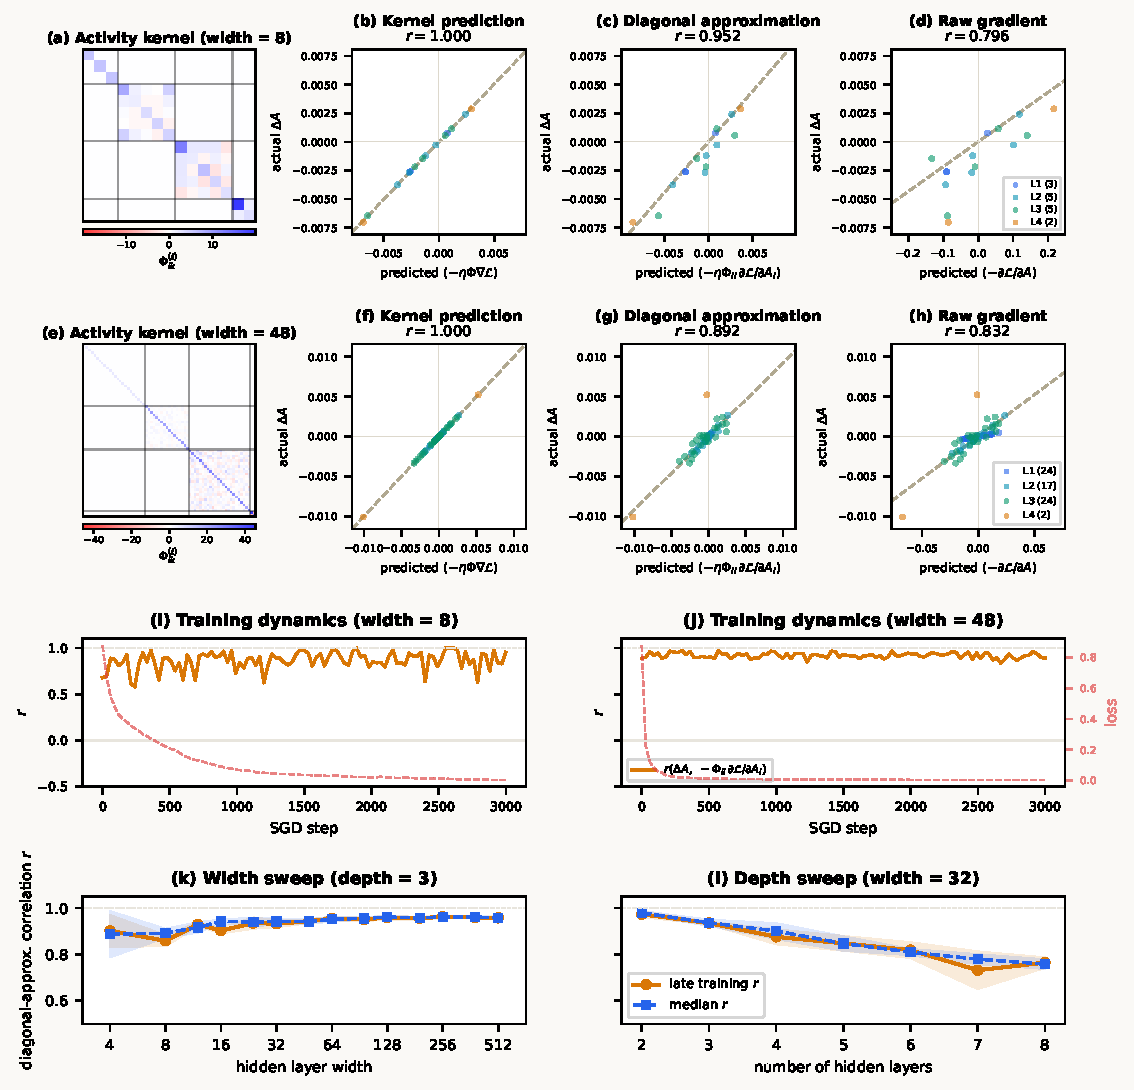
\includegraphics[width=\linewidth]{fig_main_compact}\vspace{-.5\baselineskip}}
\end{figure}

\clearpage
\bibliography{activity_dynamics}

\newpage

\appendix
\section{Experimental details}
\label{app:experimental-details}

We use fully connected multilayer perceptrons with ReLU hidden units, the same width in every hidden layer, and a two-dimensional linear output.
For an example $(\vA^{(0)},\vy)$, the loss is $\loss=\tfrac12\lVert\vA^{(L)}-\vy\rVert^2$.
Each online-SGD step samples one training example uniformly with replacement and uses learning rate $\eta=0.005$.

The training set contains 40 noisy $4\times4$ horizontal- or vertical-bar images (20 per class).
Each image has one randomly selected row or column set to one, with independent Gaussian pixel noise of standard deviation $0.15$ added to all 16 pixels.
Weights are initialised independently as $W_{ij}^{(\ell)}\sim\mathcal{N}(0,2/n_{\ell-1})$, and biases are initialised to zero.

The representative width-8 and width-48 networks have three hidden layers and are trained for 3000 steps.
Diagnostics are recorded every 30 steps and at the final step.
For each diagnostic, the activities before and after the SGD update are evaluated on the same sampled example used for that update.
The width sweep ranges from 4 to 512 at fixed depth 3, and the depth sweep ranges from 2 to 8 at fixed width 32.
Each sweep uses ten matched random replicates trained for 2000 steps, with diagnostics every 40 steps and at the final step.
Within each replicate and sweep, every architecture receives the same generated dataset and sequence of sampled-example indices.

Each Pearson correlation pools the active hidden units and both output units for one diagnostic; hidden ReLU units that are inactive before the update are excluded.
For each architecture and replicate, we take the median correlation across diagnostic steps.
The sweep curve is the mean of these ten replicate medians, and its band shows one sample standard deviation across replicates ($\mathrm{ddof}=1$).

Analysis code is available in an \href{https://anonymous.4open.science/r/activity-descent-973C/README.md}{anonymized GitHub repository}.

\section{Kernel recursion and self/cross decomposition}
\label{app:kernel-recursion}

Consider a fully connected sequential network, initially omitting biases for clarity:
\[
  z_i^{(\ell)}
  = \sum_{m\in\mathcal N_{\ell-1}} W_{im}^{(\ell)}A_m^{(\ell-1)},
  \qquad
  A_i^{(\ell)}=\sigma_\ell\!\bigl(z_i^{(\ell)}\bigr).
\]
Here $i,j,p\in\mathcal N_\ell$ index neurons in layer~$\ell$, while $m,n\in\mathcal N_{\ell-1}$ index neurons in the preceding layer.
Define the inter-layer Jacobian and the kernel contribution from layer~$\ell$'s own weights by
\[
  J_{\ell,im}
  := \frac{\partial A_i^{(\ell)}}{\partial A_m^{(\ell-1)}}
  = \sigma_\ell'\!\bigl(z_i^{(\ell)}\bigr)W_{im}^{(\ell)},
  \qquad
  D_{\ell,ij}
  := \delta_{ij}\,[\sigma_\ell'\!\bigl(z_i^{(\ell)}\bigr)]^2
  \lVert\vA^{(\ell-1)}\rVert^2.
\]
The matrix $D_\ell$ is diagonal because different neurons in a fully connected layer have disjoint incoming weight parameters.
With trainable biases, as in the experiments, $\lVert\vA^{(\ell-1)}\rVert^2$ is replaced by $\lVert\vA^{(\ell-1)}\rVert^2+1$; the contribution remains diagonal.

For an earlier weight $W_\alpha$ with $\alpha\in\mathcal P_{\leq\ell-1}$, the chain rule gives
\[
  \frac{\partial A_i^{(\ell)}}{\partial W_\alpha}
  = \sum_{m\in\mathcal N_{\ell-1}}
  J_{\ell,im}\,
  \frac{\partial A_m^{(\ell-1)}}{\partial W_\alpha}.
\]
Splitting the kernel sum into the current layer and all earlier layers therefore yields
\begin{equation}\label{eq:phi-recursion-app}
  \Phi^{(\ell)}
  = D_\ell + J_\ell\Phi^{(\ell-1)}J_\ell^\top,
  \qquad
  \Phi^{(1)}=D_1.
\end{equation}
If
\[
  J_{\ell\leftarrow r}
  := J_\ell J_{\ell-1}\cdots J_{r+1},
  \qquad
  J_{\ell\leftarrow\ell}:=I,
\]
then unrolling Equation~\eqref{eq:phi-recursion-app} gives the compact decomposition
\[
  \Phi^{(\ell)}
  = \sum_{r=1}^{\ell}
  J_{\ell\leftarrow r}\,D_r\,J_{\ell\leftarrow r}^{\top}.
\]
Every summand is positive semidefinite.
The direct term $D_\ell$ is diagonal, whereas the transported terms can contain off-diagonal entries because different neurons in layer~$\ell$ depend on shared earlier-layer parameters.

For example, at layer~2,
\[
  \Phi_{ii}^{(2)}
  = D_{2,ii}+\sum_m J_{2,im}^2D_{1,mm},
  \qquad
  \Phi_{ij}^{(2)}
  = \sum_m J_{2,im}D_{1,mm}J_{2,jm}
  \quad (j\neq i).
\]
Writing $g_j^{(2)}:=\partial\loss/\partial A_j^{(2)}$, the corresponding activity update separates into
\begin{equation}\label{eq:self-cross-app}
  \Delta A_i^{(2)}
  \approx
  -\eta\,\Phi_{ii}^{(2)}g_i^{(2)}
  -\eta\sum_{j\neq i}\Phi_{ij}^{(2)}g_j^{(2)}.
\end{equation}
Because $\Phi_{ii}^{(2)}\geq0$, the first term is aligned with neuron $i$'s negative loss gradient.
The second term mixes gradients from other neurons through their shared upstream parameter dependence and is the source of cross-neuron interference.

For smooth pointwise nonlinearities, the recursion is the usual first-order expansion in~$\eta$.
For ReLU and other piecewise-linear nonlinearities, it holds away from kinks and for finite updates that remain within the same activation region.
If an update crosses a kink, the activation-status change contributes approximation error that is not generally resolved by choosing an arbitrary subgradient.

Finally, diagonality of $D_\ell$ relies on the unshared incoming parameters of a fully connected layer.
For a differentiable sequential module with parameter sharing, such as a convolution, let $K_\ell^{\mathrm{own}}$ denote the kernel contribution from that module's own parameters; it need not be diagonal.
The recursion generalises to
\[
  \Phi^{(\ell)}
  = K_\ell^{\mathrm{own}}
  + J_\ell\Phi^{(\ell-1)}J_\ell^\top.
\]
The kernel definition and first-order activity-update relation remain valid for differentiable sequential architectures without paths that bypass layer~$\ell$.

\end{document}
